\documentclass[bachelor, och, labwork]{shiza}
% параметр - тип обучения - одно из значений:
%    spec     - специальность
%    bachelor - бакалавриат (по умолчанию)
%    master   - магистратура
% параметр - форма обучения - одно из значений:
%    och   - очное (по умолчанию)
%    zaoch - заочное
% параметр - тип работы - одно из значений:
%    referat    - реферат
%    coursework - курсовая работа (по умолчанию)
%    diploma    - дипломная работа
%    pract      - отчет по практике
% параметр - включение шрифта
%    times    - включение шрифта Times New Roman (если установлен)
%               по умолчанию выключен
\usepackage{subfigure}
\usepackage{tikz,pgfplots}
\pgfplotsset{compat=1.5}
\usepackage{float}

%\usepackage{titlesec}
\setcounter{secnumdepth}{4}
%\titleformat{\paragraph}
%{\normalfont\normalsize}{\theparagraph}{1em}{}
%\titlespacing*{\paragraph}
%{35.5pt}{3.25ex plus 1ex minus .2ex}{1.5ex plus .2ex}

\titleformat{\paragraph}[block]
{\hspace{1.25cm}\normalfont}
{\theparagraph}{1ex}{}
\titlespacing{\paragraph}
{0cm}{2ex plus 1ex minus .2ex}{.4ex plus.2ex}

% --------------------------------------------------------------------------%


\usepackage[T2A]{fontenc}
\usepackage[utf8]{inputenc}
\usepackage{graphicx}
\graphicspath{ {./images/} }
\usepackage{tempora}

\usepackage[sort,compress]{cite}
\usepackage{amsmath}
\usepackage{amssymb}
\usepackage{amsthm}
\usepackage{fancyvrb}
\usepackage{listings}
\usepackage{listingsutf8}
\usepackage{longtable}
\usepackage{array}
\usepackage[english,russian]{babel}

\usepackage[colorlinks=false]{hyperref}
\usepackage{url}

\usepackage{underscore}
\usepackage{setspace}
\usepackage{indentfirst} 
\usepackage{mathtools}
\usepackage{amsfonts}
\usepackage{enumitem}
\usepackage{tikz}
\usepackage{minted}

\newcommand{\eqdef}{\stackrel {\rm def}{=}}
\newcommand{\specialcell}[2][c]{%
\begin{tabular}[#1]{@{}c@{}}#2\end{tabular}}

\renewcommand\theFancyVerbLine{\small\arabic{FancyVerbLine}}

\newtheorem{lem}{Лемма}

\begin{document}

% Кафедра (в родительном падеже)
\chair{теоретических основ компьютерной безопасности и криптографии}

% Тема работы
\title{Отношение эквивалентности и отношение порядка}

% Курс
\course{3}

% Группа
\group{331}

% Факультет (в родительном падеже) (по умолчанию "факультета КНиИТ")
\department{факультета КНиИТ}

% Специальность/направление код - наименование
%\napravlenie{09.03.04 "--- Программная инженерия}
%\napravlenie{010500 "--- Математическое обеспечение и администрирование информационных систем}
%\napravlenie{230100 "--- Информатика и вычислительная техника}
%\napravlenie{231000 "--- Программная инженерия}
\napravlenie{10.05.01 "--- Компьютерная безопасность}

% Для студентки. Для работы студента следующая команда не нужна.
% \studenttitle{Студентки}

% Фамилия, имя, отчество в родительном падеже
\author{Токарева Никиты Сергеевича}

% Заведующий кафедрой
% \chtitle{} % степень, звание
% \chname{}

%Научный руководитель (для реферата преподаватель проверяющий работу)
\satitle{аспирант} %должность, степень, звание
\saname{В. Н. Кутин}

% Руководитель практики от организации (только для практики,
% для остальных типов работ не используется)
% \patitle{к.ф.-м.н.}
% \paname{С.~В.~Миронов}

% Семестр (только для практики, для остальных
% типов работ не используется)
%\term{8}

% Наименование практики (только для практики, для остальных
% типов работ не используется)
%\practtype{преддипломная}

% Продолжительность практики (количество недель) (только для практики,
% для остальных типов работ не используется)
%\duration{4}

% Даты начала и окончания практики (только для практики, для остальных
% типов работ не используется)
%\practStart{30.04.2019}
%\practFinish{27.05.2019}

% Год выполнения отчета
\date{2022}

\maketitle

% Включение нумерации рисунков, формул и таблиц по разделам
% (по умолчанию - нумерация сквозная)
% (допускается оба вида нумерации)
% \secNumbering

%-------------------------------------------------------------------------------------------

\section{Постановка задачи}

    \textbf{Цель работы} - изучение основных свойств бинарных отношений и операций замыкания бинарных отношений. 

    Порядок выполнения работы:
    \begin{enumerate}
        \item Разобрать определения отношения эквивалентности, фактор-множества. Разработать алгоритмы построения
        эквивалентного замыкания бинарного отношения и системы представителей фактор-множества.
        \item Разобрать определения отношения порядка и диаграммы Хассе. Разработать алгоритмы вычисления минимальных
        (максимальных) и наименьших (наибольших) элементов  и построения диаграммы Хассе.
        \item Разобрать определения контекста и концепта. Разработать алгоритм вычисления решетки концептов.
    \end{enumerate}

\section{Теоретические сведения по рассмотренным темам с их обоснованием}

    \subsection{Определение отношения эквивалентности и фактор-множества}

        Бинарное отношение $\varepsilon$ на множестве $A$ называется отношением эквивалентности (или просто эквивалентностью), если оно рефлексивно, симметрично и транзитивно.

        Для любого подмножества $X \subset A$ множество $\rho(X) = \{b \in B: (x, b) \in \rho \text{ для некоторого } x \in X\}$ называется образом множества $X$ относительно отношения $\rho$.

        Образ одноэлементного множества $X = \{a\}$ относительно отношения $\rho$ обозначается символом $\rho(a)$ и называется также образом элемента $a$ или \textbf{срезом} отношения $\rho$ через элемент $a$. 

        Срезы $\varepsilon(a)$ называются классами эквивалентности по отношению $\varepsilon$ и сокращенно обозначаются символом $[a]$. Множество всех таких классов эквивалентности $\{[a]: a \in A\}$ называется фактор-множеством множества $A$ по эквивалентности $\varepsilon$ и обозначается символом $A/\varepsilon$.

        Подмножество $T \subset A$ называется \textbf{полной системой представителей классов} эквивалентности $\varepsilon$ на множестве $A$, если:
        
        \begin{itemize}
            \item $\varepsilon(T) = A$;
            \item из условия $t_1 \equiv t_2(\varepsilon)$ следует $t_1 = t_2$.
        \end{itemize}

        Классы эквивалентности $[t] \in A/\varepsilon$ могут быть отождествлены со своими представителями $t$ и фактор-множество $A/\varepsilon$ 
        может быть отождествлено с множеством $T$.

        \textbf{Лемма 1.} О замыканиях бинарных отношений.

        На множестве $P(A^2)$ всех бинарных отношений между элементами множества $A$ следующие отображения являются
        операторами замыканий:

        \begin{enumerate}
            \item $f_r(\rho) = \rho \cup \triangle_A$ - наименьшее рефлексивное бинарное отношение, содержащее отношение
            $\rho \subset A^2$,
            \item $f_s(\rho) = \rho \cup \rho^{-1}$ - наименьшее симметричное бинарное отношение, содержащее отношение
            $\rho \subset A^2$,
            \item $f_t(\rho) = \bigcup^\infty_{n=1} \rho^{n}$ - наименьшее транзитивное бинарное отношение, содержащее
            отношение $\rho \subset A^2$,
            \item $f_{eq}(\rho) = f_t f_s f_r(\rho)$ - наименьшее отношение эквивалентности, на содержащее отношение
            $\rho \subset A^2$.
        \end{enumerate}        

    \subsection{Определение отношения порядка}

        Бинарное отношение $\omega$ на множестве $A$ называется отношением порядка (или просто порядком), если оно
        рефлексивно, антисимметрично и транзитивно.

        Множество $A$ с заданным на нем отношением порядка $\leq$ называется упорядоченным множеством и обозначается $A
        = (A, \leq)$ или просто $(A, \leq)$.

        Элемент $a$ упорядоченного множества $(A, \leq)$ называется:
        \begin{enumerate}
            \item минимальным, если $(\forall x \in A) \text{ } x \leq a \implies x = a$,
            \item максимальным, если $(\forall x \in A) \text{ } a \leq x \implies x = a$,
            \item наименьшим, если $(\forall x \in A) \text{ } a \leq x$,
            \item наибольшим, если $(\forall x \in A) \text{ } x \leq a$.
        \end{enumerate}

        \textbf{Лемма 2.}

        Для любого конечного упорядоченного множества $A = (A, \leq)$ справедливы следующие утверждения:
        \begin{enumerate}
            \item любой элемент множества $A$ содержится в некотором максимальном элементе и содержит некоторый
            минимальный элемент;
            \item если упорядоченное множество $A$ имеет один максимальный (соответственно, минимальный) элемент, то он
            является наибольшим (соответственно, наименьшим) элементом этого множества.
        \end{enumerate}

    \subsection{Определение диаграммы Хассе}

        Упорядоченное множество $A = (A, \leq)$ наглядно представляется диаграммой Хассе, которая представляет элементы множества $A$ точками 
        плоскости и пары $a <\cdot \text{ } b$ представляет линиями, идущими вверх от элемента $a$ к элементу $b$.

        Стоит отметить, что запись $a <\cdot \text{ } b$, означает, что $a \leq b$ и нет элементов x, удовлетворяющих условию $a < x < b$.
        В этом случае говорят, что элемент $b$ покрывает элемент $a$ или что элемент $a$ покрывается элементом $b$.
        
        Алгоритм построения диаграммы Хассе конечного упорядоченного множества $A = (A, \leq)$.

        \begin{enumerate}
            \item В упорядоченном множестве $A = (A, \leq)$ найти множество $A_1$ всех минимальных элементов и расположить их в один горизонтальный ряд (это первый уровень диаграммы).
            \item В упорядоченном множестве $A \setminus A_1$, найти множество $A_2$ всех минимальных элементов и
            расположить их в один горизонтальный ряд над первым уровнем (это второй уровень диаграммы). Соединить
            отрезками элементы этого ряда с покрываемыми ими элементами предыдущего ряда.
            \item В упорядоченном множестве $A \setminus (A_1 \cup A_2)$ найти множество $A_3$ всех минимальных
            элементов и расположить их в один горизонтальный ряд над вторым уровнем (это третий уровень диаграммы).
            Соединить отрезками элементы этого ряда с покрываемыми ими элементами предыдущих рядов.
            \item Процесс продолжается до тех пор, пока не выберутся все элементы множества $A$.
        \end{enumerate}

    \subsection{Определение контекста и концепта}

        Контекстом называется алгебраическая система $K = (G, M, \rho)$, состоящая из множества объектов $G$, множества атрибутов $M$ и бинарного отношения $\rho \subset G \times M$, показывающего $(g, m) \in \rho$, что объект $g$ имеет атрибут $m$.

        Упорядоченная пара $(X, Y)$ замкнутых множеств $X \in Z_{f_G}, Y \in Z_{f_M}$, удовлетворяющих условиям $\varphi(X) = Y$, $\psi(Y) = X$, называется концептом контекста $K = (G, M, \rho)$. При этом компонента $X$ называется объемом и компонента $Y$ - содержанием концепта $(X, Y)$.

        Множество всех концептов $C(K)$ так упорядочивается отношением \\ $(X, Y) \leq (X_1, Y_1) \Leftrightarrow X \subset X_1$ (или равносильно $Y_1 \subset Y$), что $(C(K), \leq)$ является полной решеткой, которая изоморфна решетке замкнутых подмножеств множества $G$.

        Алгоритм вычисления системы замыканий на множестве $G$:
        \begin{enumerate}
            \item Рассматриваем множество $G \in Z_{f_G}$.
            \item Последовательно перебираем все элементы $m \in M$ и вычисляем для них $\psi(\{m\}) = \rho^{-1}(m)$.
            \item Вычисляем все новые пересечения множества $\psi(\{m\})$ с ранее полученными множествами и добавляем новые множества к $Z_{f_G}$. Аналогично вычисляется система замыканий на множестве $M$.
        \end{enumerate}

\section{Результаты работы}
    \subsection{Описание алгоритма построения эквивалентного замыкания бинарного отношения и системы представителей
    фактор-множества}

        \underline{Алгоритм 1 - Построение эквивалентного замыкания}\\
            \textit{Вход}: Матрица бинарного отношения $A = (a_{ij})$ размерности $n \times n$.\\
            \textit{Выход}: Исходная матрица бинарного отношения, замкнутая относительно рефлексивности, симметричности и
            транзитивности.\\
            \underline{Шаг 1.} Построить рефлексивное замыкание на матрице $A = (a_{ij})$ бинарного отношения.
            Необходимо пройти по всем элементам $a_{ii}$ матрицы $A$, где $0 \leq i < n$, и присвоить им единицу (т.е. $a_{ii}=1$).\\
            \underline{Шаг 2.} Выполнив шаг 1, построить симмтеричное замыкание на матрице $A$ бинарного отношения. 
            Необходимо пройти по всем элементам  $a_{ij}$ матрицы $A$, где $0 \leq i,j < n$ Если элемент $a_{ij}=1$,
            а элемент $a_{ji} \neq 1$, то нужно присвоить $a_{ji}$ единицу.\\            
            \underline{Шаг 3.} Выполнив шаг 2, построить транзитивное замыкание на матрице $A$ бинарного отношения.
            Если $a_{ik} = 1 \wedge a_{kj} = 1$, то нужно приравнять $a_{ij}$ к единице, где $a_{ik}$, $a_{kj}$, $a_{ij}$ --
            элементы матрицы $A$, ($0 \leq i,j,k < n$). Данная процедура должна повторится n раз согласно пункту 3 леммы 1 
            (о замыканиях бинарных отношений), где говорится об операторе транзитивного замыкания.\\
            \underline{Шаг 4.} Вернуть полученную матрицу $A = (a_{ij})$ бинарного отношения, замкнутой относительно 
            рефлексивности, симметричности и транзитивности.\\
            
            Оценка сложности данного алгоритма равна $O(n + n^2 + n^4) = O(n^4)$.\\

        \underline{Алгоритм 2 - Построение системы представителей фактор-множества}\\
            \textit{Вход}: Матрица бинарного отношения $A = (a_{ij})$ размерности $n \times n$.\\
            \textit{Выход}: Список $repsys$, в котором содержатся числа, составляющие систему представителей 
            $T$ фактор-множества $X/\varepsilon$ бинарного отношения на множестве $X$.\\
            \underline{Шаг 1.} Создать пустые списокы $tmp = []$, $fset = []$ и $repsys = []$.\\ 
            \underline{Шаг 2.} Необходимо построить фактор-множество $X/\varepsilon$, получив срезы по каждому элементу $a \in X$.
            Для этого нужно проверить элементы $a_{ij}$ матрицы $A$. Если $a_{ij} = 1$, где $0 \leq i, j < n$, то добавить значение $j$
            в список $tmp$. \\ 
            \underline{Шаг 3.} Если полученного списка $tmp$ нет в списке $fset$, то добавить его в список $fset$, в противном
            случае -- не добавлять.\\
            \underline{Шаг 4.} Найти в каждом подсписке $fset[i]$ ($0 \leq i < k$) списка $fset$ минимум $el_{min}$, и затем добавить
            в список $repsys$ пару ($el_{min}$, $fset[i]$). \\
            \underline{Шаг 5.} Вернуть список $repsys$ в качестве выхода функции. \\
            
            Оценка сложности данного алгоритма состоит из оценки сложности формирования списка $fset$ равной $O(n^2)$ и оценки сложности
            нахождения минимума для формирования списка $repsys$ равной $O(n^2)$. В итоге получаем оценку: $O(n^2 + n^2) = O(n^2)$.\\

    \subsection{Описание  алгоритмов  вычисления  минимальных  (максимальных)  и  наименьших (наибольших) элементов и
    построения диаграммы Хассе}

        \underline{Алгоритм 3 - Вычисление минимального элемента множества} \\
            \textit{Вход}: Матрица бинарного отношения $A = (a_{ij})$ размерности $n \times n$ и список $set_x$, состоящий из элементов
            множества $X$, и  число $k$.\\            
            \textit{Выход}: Список $L_{min}$, значения которого являются минимальными элементами упорядоченного множества $(X, \leq)$.\\
            \underline{Шаг 1.} Создать пустой список $L_{min} = []$.\\
            \underline{Шаг 2.} Создать цикл с индексом $i$, где $k \leq i < n$, в котором инициализировать булеву переменную $fl = true$.
            Затем создать вложенный цикл с индексом $j$, где $k \leq j < n$, в котором поставить условие. Если $a[i][j] \neq 0 \wedge i \neq j$,
            то булевой переменной присвоить $fl = false$. \\
            \underline{Шаг 3.} Если после завершения вложенного цикла с индексом $j$ значение флага не изменилось (т.е. $fl = true$), то
            добавить в список $L_{min}$ значение $set_x[j]$.\\
            \underline{Шаг 4.} Вернуть список $L_{min}$ в качестве выхода функции.\\

            Оценка сложности данного алгоритма равна $O(n^2)$.\\

        \underline{Алгоритм 4 - Вычисление максимального элемента множества}\\
            \textit{Вход}: Матрица бинарного отношения $A = (a_{ij})$ размерности $n \times n$ и список $set_x$, состоящий из элементов
            множества $X$, и число $k$.\\            
            \textit{Выход}: Список $L_{max}$, значения которого являются максимальными элементами упорядоченного множества $(X, \leq)$.\\
            \underline{Шаг 1.} Создать пустой список $L_{max} = []$.\\
            \underline{Шаг 2.} Создать цикл с индексом $i$, где $k \leq i < n$, в котором инициализировать булеву переменную $fl = true$.
            Затем создать вложенный цикл с индексом $j$, где $k \leq j < n$, в котором поставить условие. Если $a[j][i] \neq 0 \wedge i \neq j$,
            то булевой переменной присвоить $fl = false$. \\
            \underline{Шаг 3.} Если после завершения вложенного цикла с индексом $j$ значение флага не изменилось (т.е. $fl = true$), то
            добавить в список $L_{max}$ значение $set_x[j]$.\\
            \underline{Шаг 4.} Вернуть список $L_{max}$ в качестве выхода функции.\\

            Оценка сложности данного алгоритма равна $O(n^2)$.\\

            

        \underline{Алгоритм 5 - Вычисление наименьшего элемента множества}\\
            \textit{Вход}: Список $L_{min}$, значения которого являются минимальными элементами упорядоченного множества $(X, \leq)$.\\
            \textit{Выход}: Наименьший элемент $x_{min}$ упорядоченного множества $(X, \leq)$ или значение -1.\\
            \underline{Шаг 1.} Если длина $L_{min}$ не равна $1$, то вернуть -1, иначе -- вернуть единственный элемент $x_{min} = l \in L_{min}$,
            являющийся наименьшим элементом множества $X$.\\
                
            Трудоемкость алгоритма $O(1)$.\\

        \underline{Алгоритм 6 - Вычисление наибольшего элемента множества}\\
            \textit{Вход}: Список $L_{max}$, значения которого являются максимальными элементами упорядоченного множества $(X, \leq)$.\\
            \textit{Выход}: Наибольший элемент $x_{max}$ упорядоченного множества $(X, \leq)$ или значение -1.\\
            \underline{Шаг 1.} Если длина $L_{max}$ не равна $1$, то вернуть -1, иначе -- вернуть единственный элемент
            $x_{max} = l \in L_{max}$, являющийся наибольшим элементом множества $X$.\\
                
            Трудоемкость алгоритма $O(1)$.\\

        \underline{Алгоритм 7 - Построение диаграммы Хассе}\\
            \textit{Вход}: Матрица бинарного отношения порядка $A = (a_{ij})$ размерности $n \times n$ и список $set_x$, 
            состоящий из элементов множества $X$.\\
            \textit{Выход}: Список $H$ длиной $n$, характеризующий диаграмму Хассе: каждый элемент в списке представляет
            собой четыре значения: элемент $x \in X$, значение его уровня $l$ на диаграмме, список $prevV$ элементов множества
            $X$, находящихся на уровне $lvl - 1$, список $nextV$ элементов множества $X$, находящихся на уровне $lvl + 1$ относительно
            элемента $x$. \\
            \underline{Шаг 1.} Инициализировать списки $diagramm = []$, $el\_and\_lvl = []$ и переменные $k = 0$, $lvl = 0$.\\
            \underline{Шаг 2.} Создать цикл, с условием, что пока $k \neq n$, где $n$ -- длина списка $set_x$. Запустить алгоритм 3, где
            в качестве входных данных подать матрицу $A$, список $set_x$ и число $k$.\\
            \underline{Шаг 3.} При завершении алгоритма 3 был получен список $L_{min}$, значения которого являются
            минимальными элементами упорядоченного множества $(X, \leq)$. Далее нужно увеличить значение переменной $lvl$ на 1. \\    
            \underline{Шаг 4.} Необходимо создать цикл, где совершается проход по всем элементам $el$ списка $L_{min}$, для того чтобы
            сформировать пару ($el$, $lvl$) и добавить её в список $el\_and\_lvl$. При добавлении нового элемента в список $el\_and\_lvl$
            увеличивается значение переменной $k$ на 1.\\
            \underline{Шаг 5.} После завершения цикла, созданного на шаге 2, необходимо создать цикл с индексом $i$ ($0 \leq i < n$), в
            котором инициализировать списки $nextV = []$ и $prevV = []$ и переменные $nextlvl = el\_and\_lvl[i][1] + 1$ 
            и $prevlvl = el\_and\_lvl[i][1] - 1$. Далее нужно создать вложенный цикл с индексом $j$ ($0 \leq j < n$), где выполняются следующие
            условия. Если $el\_and\_lvl[j][1] = nextlvl$, то добавить в список $nextV$ элемент $el\_and\_lvl[j][0]$. Если 
            $el\_and\_lvl[j][1] = prevlvl$, то добавить в список $prevV$ элемент $el\_and\_lvl[j][0]$. \\
            \underline{Шаг 6.} С учетом предыдущих шагов, нужно добавить в список $diagramm$ следующий кортеж: ($el\_and\_lvl[j][0]$, $el\_and\_lvl[j][1]$,
            $prevV$, $nextV$). \\
            \underline{Шаг 7.} Вернуть полученный список $diagramm$ в качестве выхода функции.\\

            Оценка сложности данного алгоритма с учётом оценки сложности построения списка $el\_and\_lvl$ равной $O(n^2)$ и с учетом оценки сложности
            построения списка $diagramm$ равной $O(n^2)$ будет равна $O(n^2 + n^2) = O(n^2)$.\\
            % \underline{Шаг 5.} Определить пустой список $V$. Проходясь по элементам списка $L$, где $0 \leq k \leq n -
            % 1$, определять для каждого значения $l_k$ пустой список $v_k$ связанных с элементом $a_k$ элементов
            % множества $A$. Определяя такой список, далее проходить по элементам $a_{ij}$ матрицы $A$, где $0 \leq i, j
            % \leq n - 1$: если значение $a_{ij} = 1$ и уровень $l_i \in L$ элемента $a_i \in A$ равен $l_k + 1$, то
            % добавить элемент $a_i$ в список $v_k$. После этого отсортировать список $v_k$ и добавить его в $V$. \\
            % \underline{Шаг 6.} Создать список $H$ и поместить в него в качестве элемента $h_i \in H$ тройку значений:
            % $a_i \in A$, $l_i \in L$, $v_i \in V$, где $0 \leq i \leq n - 1$. После этого вернуть список $H$. \\

            % Трудоемкость алгоритма $O(n^3)$.\\

    \subsection{Описание алгоритма построения решетки концептов}

        \underline{Алгоритм 8 - Построение системы замыканий}\\
            \textit{Вход}: Список $objs$, который содержит $n$ элементов множества объектов $G$, список $attrs$, 
            который содержит $k$ элементов множества объектов $M$ и матрица $A = (a_{ij})$ бинарного отношения
            $\rho \subset G \times M$ размерности $n \times k$. \\
            \textit{Выход}: Список $set_z$, значения которого являются элементы системы замыканий $Z_{f_G}$
            на множестве $G$.\\
            \underline{Шаг 1.} Создать список $set_z$ и добавить в него список $objs$ в качестве первого элемента.\\
            \underline{Шаг 2.} Создать цикл с индексом $i$, где $0 \leq i < k$, в котором инициализировать пустой список $cur\_slice = []$.
            Затем создать вложенный цикл с индексом $j$, где $0 \leq j < n$, в котором поставить условие. Если $a[j][i] = 1$, то добавить
            в список $cur\_slice$ значение $objs[j]$.\\
            \underline{Шаг 3.} Далее необходимо сделать пересечение полученного множества $cur\_slice$ с каждым элементом из множества
            $set_z$. Обозначим текущее пересечение, как $x \in set_z$. Если элемент $x$ не содержится в данном множестве (списке) $set_z$,
            то его следует добавить в список $set_z$, иначе пропустить.\\
            \underline{Шаг 4.} Вернуть список $set_z$ в качестве выхода функции.\\ 
            
            Оценка сложности данного алгоритма равна $O(n \cdot k + n^2)$.
            % Получить срезы по атрибутам $m \in M$ с помощью способа, описанного в алгоритме 2:
            % необходимо предварительно транспонировать матрицу $B = A^T = (a_{ij})^T = b_{ij}$, затем проверить элементы
            % $b_{ij}$ матрицы $B$, и если $b_{ij} = 1$, где $0 \leq i \leq k - 1$ и $0 \leq j \leq n - 1$, то добавить
            % значение объекта $g_j$ в список, определяющий срез по атрибуту $m_i$. В результате получить список срезов
            % $S_G = \{s_i = [g]: g \in G\}$, размер которого будет $k$. \\
            % \underline{Шаг 3.} Для каждого атрибута $m_i \in M$: определить список $T$, в который поместить $s_i \in
            % S_G$. Далее для каждого замыкания $z_j$ из системы замыканий $Z_{f_G}$: получить пересечение множеств $s_i$
            % и $z_j$ и обозначить его как $X = s_i \cap z_j$. Если $X$ не содержится в списке $T$: добавить $X$ в список
            % $T$ (всё это осуществляется при $0 \leq i \leq k - 1$). Если $T \notin Z_{f_G}$, то положить $T$ в
            % $Z_{f_G}$.\\
            % \underline{Шаг 4.} Вернуть систему замыканий $Z_{f_G}$ на множестве $G$.\\

            % Трудоемкость алгоритма $O(n^2 + n \cdot k)$.\\

        \underline{Алгоритм 9 - Построение решетки концептов}\\
            \textit{Вход}: Список $set_z$, значения которого являются элементы системы замыканий $Z_{f_G}$
            на множестве $G$. Список $objs$, содержащий $n$ элементов множества объектов $G$, список $attrs$, 
            который содержит $k$ элементов множества объектов $M$ и матрица $A = (a_{ij})$ бинарного отношения
            $\rho \subset G \times M$ размерности $n \times k$. \\
            \textit{Выход}: список $set\_isomorph$, который содержит элементы решетки концептов $(C(K), \leq)$. \\
            \underline{Шаг 1.} Инициализировать словарь $tmp\_iso = {}$, где ключами будут являться элементы
            $objs[i]$ ($0 \leq i < n$), а значениями -- список элементов, который формируется на шаге 2.\\
            \underline{Шаг 2.} Создать цикл с индексом $i$, где $0 \leq i < n$, в котором инициализировать
            пустой список $cur\_slice = []$. Далее создать вложенный цикл с индексом $j$, где $0 \leq j < k$,
            в котором поставить условие. Если $a[j][i] = 1$, то добавить в список $cur\_slice$ значение $attrs[j]$.
            Затем необходимо добавить в словарь элемент, где ключом будет являться $objs[i]$, а значением -- список
            $cur\_slice$. \\ 
            \underline{Шаг 3.} Инициализировать список $set\_isomorph = []$. Далее, проходя по всем спискам $el$, принадлижащих
            списку $set_z$, производится пересечение элементов $tmp\_iso[el[i]]$ ($0 \leq i < l$, где $l$ - длина списка $el$),
            которую обозначим $intersec$.
            \underline{Шаг 4.} Формируем пару ($arg_1, arg_2$), где $arg_1$ -- текущий список $el$, $arg_2$ -- пересечение
            $intersec$. Такую пару добавляем в список $set\_isomorph$. В конечном итоге получаются элементы решетки
            концептов $(C(K), \leq)$.\\
            \underline{Шаг 5.} Вернуть полученный список $set\_isomorph$ в качестве выхода функции.\\

            Оценка сложности данного алгоритма состоит из оценки сложности прохождения по элементам $a_{ij}$ матрицы $A$ 
            ($0 \leq i < n$, $0 \leq j < k$), равной $O(n \cdot k)$ и оценки сложности прохождения по всем элементам списка $set_z$,т.е.
            $O(m \cdot n)$, где $m$ -- количество элементов списка $set_z$. Тогда оценка сложности равна: $O(n \cdot (k + m))$.\\

    \subsection{Коды программ, реализующей рассмотренные алгоритмы}


        \inputminted[fontsize=\small]{Python}{code/aua-lab2.py}








    \subsection{Результаты тестирования программ}
    
        \begin{figure}[H]
            \centering
            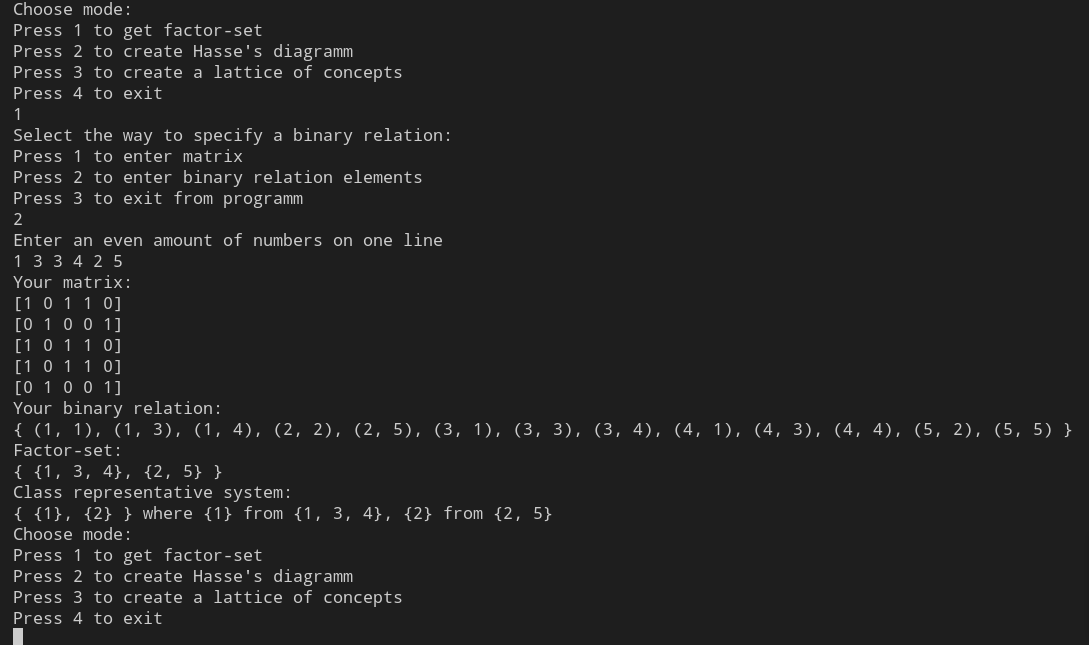
\includegraphics[width=0.8\textwidth]{photo/1.png}
            \caption{Тест алгоритма построения эквивалентного замыкания}
        \end{figure}

        \begin{figure}[H]
            \centering
            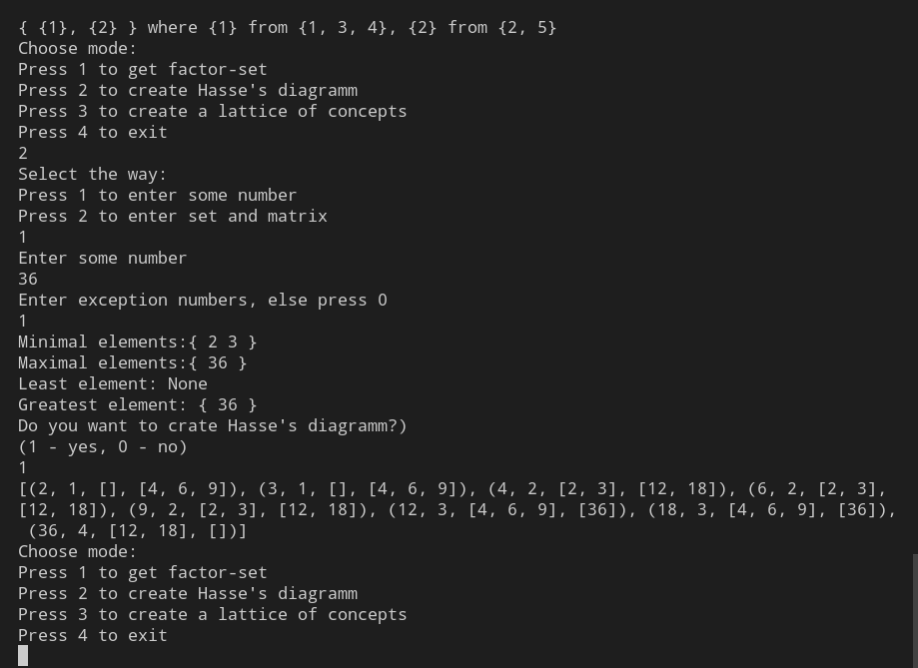
\includegraphics[width=1\textwidth]{photo/2.png}
            \caption{Тест алгоритма построения диаграммы Хассе на множестве ($X$, $|$)}
        \end{figure}

        \begin{figure}[H]
            \centering
            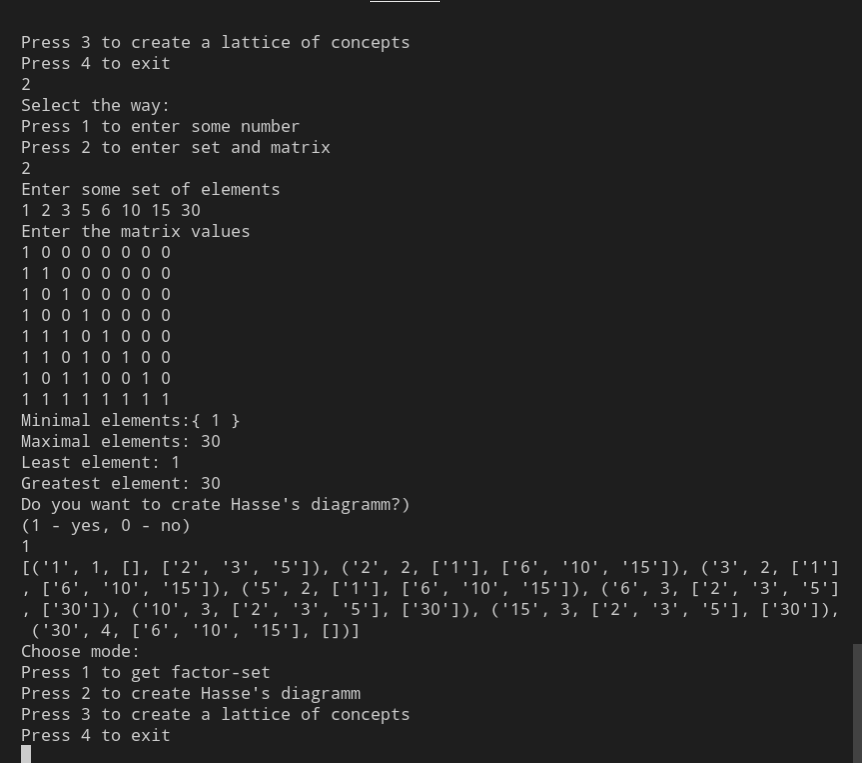
\includegraphics[width=1\textwidth]{photo/3.png}
            \caption{Тест алгоритма построения диаграммы Хассе на множестве ($X$, $\leq$)}
        \end{figure}

        \begin{figure}[H]
            \centering
            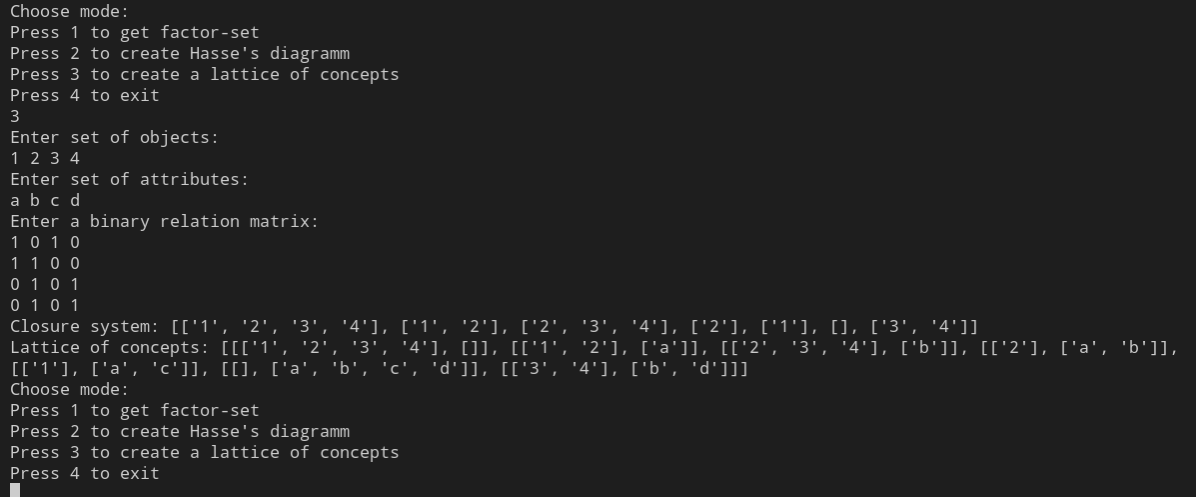
\includegraphics[width=1\textwidth]{photo/4.png}
            \caption{Тест алгоритма построения решетки концепта}
        \end{figure} 
    \newpage
 
    \conclusion
    
    В результате лабораторной работы были рассмотрены теоретические сведения об отношении эквивалентности, разобраны
    определения фактор-множества, отношения порядка и диаграммы Хассе, контекста и концепта. Опираясь на изложенную
    выше теорию, были разработаны алгоритмы построения эквивалентного замыкания бинарного отношения и системы представителей
    фактор-множества, алгоритмы вычисления минимальных (максимальных) и наименьших (наибольших) элементов и построения
    диаграммы Хассе, а также алгоритмы построения решетки концептов. Была произведена оценка сложности каждого из 
    построенных алгоритмов. Была реализована программа, написанная на языке Python.
    
\end{document}